\documentclass[14pt]{beamer}

\mode<presentation>{ \usetheme{Madrid}

% To remove the navigation symbols from the bottom of all slides uncomment next line
\setbeamertemplate{navigation symbols}{}
\date{}
\title{}
\author{}

%to get rid of footer entirely uncomment next line
\setbeamertemplate{footline}{}
}

\usepackage{geometry}
\usepackage{multirow}
\usepackage{adjustbox}
\usepackage{multicol}
\setlength{\columnsep}{0.1cm}

\usepackage{tikz}
\usetikzlibrary{shapes, backgrounds}

\usepackage{bbding}
\usepackage{rotating}
\usepackage{xcolor}

%\usepackage{tkz-berge} %cool grid
\usepackage{pgfplots} %pics

\usepackage{graphicx} % Allows including images
\usepackage{
	booktabs
} % Allows the use of \toprule, \midrule and \bottomrule in tables
\usepackage{mathtools}

\newcommand{\R}{\mathbb{R}}
\newcommand{\Z}{\mathbb{Z}}
\newcommand{\N}{\mathbb{N}}
\newcommand{\e}{\varepsilon}

\newcommand{\p}{% \pause
}

% simple environrment for enumerate, easier to read
\setbeamertemplate{enumerate items}[default]

%%%%%%%%%%%%%%%%%%%%%%

% to use colours easily
\definecolor{verde}{rgb}{0, .7, 0}
\definecolor{rosa}{rgb}{1, 0, 1}
\definecolor{naranja}{rgb}{1, .5, 0.1}
\newcommand{\azul}[1]{{\color{blue} #1}}
\newcommand{\rojo}[1]{{\color{red} #1}}
\newcommand{\verde}[1]{{\color{verde} #1}}
\newcommand{\rosa}[1]{{\color{rosa} #1}}
\newcommand{\naranja}[1]{{\color{naranja} #1}}
\newcommand{\violeta}[1]{{\color{violet} #1}}

% box in red and blue in math and outside of math
\newcommand{\cajar}[1]{\boxed{\mbox{\rojo{ #1}}}}
\newcommand{\majar}[1]{\boxed{\rojo{ #1}}}
\newcommand{\cajab}[1]{\boxed{\mbox{\azul{ #1}}}}
\newcommand{\majab}[1]{\boxed{\azul{ #1}}}

\newcommand{\setsize}[1]{\fontsize{#1}{#1}\selectfont} %allows you to change the font size. The default size of this document is 14. To change the font size of the whole slide, place this at the beginning of the slide. To change the size of only a portion of the text to size 12, you can do the following { \setsize{12} Your text. }.

\setbeamerfont{frametitle}{size=\fontsize{15}{15}\selectfont}
\setbeamerfont{block title}{size=\fontsize{14}{14}\selectfont}

\newcommand{\smallerfont}{\setsize{13}} %place this at the beginning of a slide to set the font size of the entire slide to 13.

%===========================

% Preamble just for this file

%===========================

\newcommand{\aaa}{\boxed{\phantom{???}}}
\newcommand{\bbb}{\boxed{\phantom{?????^f_p}}}
\newcommand{\lifab}{\underline{I_a^b}(f)}
\newcommand{\uifab}{\overline{I_a^b}(f)}
\newcommand{\puntos}[2]{ \draw[thick] (-5,0) to (5,0);

\draw[decorate, decoration={brace, amplitude=10pt}, yshift=10pt] (#1-3.5,-0) -- (#1-0,-0)
node [red,midway,yshift=20pt]{lower sums};

\draw[red, fill] (#1-2.5,0) circle [radius=0.1] ; \draw[red, fill] (#1-3.3,0)
circle [radius=0.1] ; \draw[red, fill] (#1-2.0,0) circle [radius=0.1] ; \draw[red,
fill] (#1-1.8,0) circle [radius=0.1] ; \draw[red, fill] (#1-1.3,0) circle [radius=0.1]
; \draw[red, fill] (#1-0.8,0) circle [radius=0.1] ; \draw[red, fill] (#1-0.5,0) circle
[radius=0.1] ; \draw[red, fill] (#1-0.2,0) circle [radius=0.1] ; \draw[red, fill]
(#1-0.05,0) circle [radius=0.1] ;

\draw[decorate, decoration={brace, amplitude=10pt}, yshift=10pt] (#2+0,0) -- (#2+3.5,0)
node [verde,midway,yshift=20pt]{upper sums};

\draw[verde, fill] (#2+2.7,0) circle [radius=0.1] ; \draw[verde, fill] (#2+3.1,0)
circle [radius=0.1] ; \draw[verde, fill] (#2+1.8,0) circle [radius=0.1] ; \draw[verde,
fill] (#2+1.5,0) circle [radius=0.1] ; \draw[verde, fill] (#2+1.2,0) circle [radius=0.1]
; \draw[verde, fill] (#2+0.7,0) circle [radius=0.1] ; \draw[verde, fill] (#2+0.4,0)
circle [radius=0.1] ; \draw[verde, fill] (#2+0.2,0) circle [radius=0.1] ; \draw[verde,
fill] (#2+0.03,0) circle [radius=0.1] ; }

\newcommand{\puntosmas}[2]{ \puntos{#1}{#2} \draw[very thick, ->] (#1-3.5,-1)--(#1-0,-1)
node[black,midway,yshift=-20pt]{finer partitions}; \draw[very thick, ->] (#2+3.5,-1)--(#2+0,-1)
node[black,midway,yshift=-20pt]{finer partitions}; }

%===================================================
\begin{document}
	%===================================================

	%----------------------------------------------------------------------------------------

	%	Sigma notation for sums

	%----------------------------------------------------------------------------------------

	%-----------------------------

	%QUESTION_INFO: {"unit":7,"question":0,"title":"Warm-up: sums","images":[]}
	\begin{frame}[t]
		\frametitle{Warm-up: sums}

		Compute

		\begin{enumerate}
			\item $\displaystyle \sum_{i=2}^{4}(2i+1)$
				\vfill

			\item $\displaystyle \sum_{i=2}^{4}2i + 1$
				\vfill

			\item $\displaystyle \sum_{j=2}^{4}(2i + 1)$
				\vfill
		\end{enumerate}
	\end{frame}
	%------------------------------

	%QUESTION_INFO: {"unit":7,"question":1,"title":"Write these sums with $\\Sigma$ notation","images":[]}
	\begin{frame}[t]
		\fontsize{13}{13}\selectfont
		\frametitle{Write these sums with $\Sigma$ notation}

		\begin{enumerate}
			\item $\displaystyle 1^{5}+ 2^{5}+ 3^{5}+ 4^{5}+ \ldots + 100^{5}$
				\vfill

			\item $\displaystyle \frac{2}{4^{2}}+ \frac{2}{5^{2}}+ \frac{2}{6^{2}}+ \frac{2}{7^{2}}
				+ \ldots + \frac{2}{N^{2}}$
				\vfill

			\item $\displaystyle \cos 0 - \cos 1 + \cos 2 - \cos 3 + %\cos 4 -
				\ldots \pm \cos (N+1)$
				\vfill

			\item $\displaystyle \frac{1}{0!}+ \frac{1}{2!}+ \frac{1}{4!}+ \frac{1}{6!}
				+ \ldots + \frac{1}{(2N)!}$
				\vfill

			\item $\displaystyle \frac{1}{1!}- \frac{1}{3!}+ \frac{1}{5!}- \frac{1}{7!}
				+ \ldots + \frac{1}{81!}$
				\vfill

			\item $\displaystyle \frac{2x^{3}}{ 4!}+ \frac{3x^{4}}{5!}+ \frac{4x^{5}}{6!}
				+ \ldots + \frac{999x^{1000}}{1001!}$
		\end{enumerate}
	\end{frame}

	%------------------------------

	%QUESTION_INFO: {"unit":7,"question":2,"title":"Re-writing sums","images":[]}
	\begin{frame}[t]
		\fontsize{13}{13}\selectfont
		\frametitle{Re-writing sums}

		\begin{enumerate}
			\item $\displaystyle \sum_{i=1}^{100}\tan i \, - \, \sum_{i=1}^{50}\tan i \;
				= \; \sum_{\boxed{\phantom{???}}}^{\boxed{\phantom{???}}}\boxed{\phantom{?????^f_p}}$
				\vfill

			\item $\displaystyle \sum_{i=1}^{N}(2i-1)^{5}\; = \; \sum_{i=0}^{N-1}\boxed
				{\phantom{?????^f_p}}$
				\vfill

			\item $\displaystyle \left[ \sum_{k=1}^{N}x^{k}\right] \, + \, \left[ \sum_{k=0}
				^{N}k \; x^{k+1}\right] \; = \; \left[ \sum_{k=\boxed{\phantom{???}}}^{\boxed{\phantom{???}}}
				\!\!\boxed{\phantom{???}}\,x^{k}\right] \, + \, \boxed{\phantom{???}}$
				\vfill
		\end{enumerate}

		\emph{Hint:} Write out the sums on the left hand side first, simplify if
		possible, then write them back into sigma notation.
	\end{frame}
	%------------------------------

	%QUESTION_INFO: {"unit":7,"question":3,"title":"Telescopic sum","images":[]}
	\begin{frame}[t]
		\frametitle{Telescopic sum}

		\begin{itemize}
			\item Calculate the exact value of
				\[
					\sum_{i=1}^{137}\left[ \frac{1}{i}- \frac{1}{i+1}\right]
				\]
				\emph{Hint:} Write down the first few terms.

			% \pause

			\item Calculate the exact value of
				\[
					\sum_{i=1}^{10,000}\frac{1}{i(i+1)}
				\]
		\end{itemize}
	\end{frame}

	%------------------------------

	%QUESTION_INFO: {"unit":7,"question":4,"title":"Double sums","images":[]}
	\begin{frame}[t]
		\frametitle{Double sums}

		Compute:
		\begin{multicols}{3}
			\begin{enumerate}
				\item $\displaystyle \sum_{i=1}^{N}\sum_{k=1}^{N}1$

				\item $\displaystyle \sum_{i=1}^{N}\sum_{k=1}^{i}1$

				\item $\displaystyle \sum_{i=1}^{N}\sum_{k=1}^{i}i$

				\item $\displaystyle \sum_{i=1}^{N}\sum_{k=1}^{i}k$

				\item $\displaystyle \sum_{i=1}^{N}\sum_{k=1}^{i}(ik)$
			\end{enumerate}
		\end{multicols}

		\vfill

		{\fontsize{10}{10}\selectfont Useful formulas: \begin{align*}&\sum_{j=1}^{N}j = \frac{N(N+1)}{2},&&\sum_{j=1}^{N}j^{2}= \frac{N(N+1)(2N+1)}{6},&&\sum_{j=1}^{N}j^{3}= \frac{N^{2}(N+1)^{2}}{4}\end{align*} }
	\end{frame}
	%------------------------------

	%QUESTION_INFO: {"unit":7,"question":5,"title":"Harmonic sums","images":[]}
	\begin{frame}[t]
		\fontsize{13}{13}\selectfont
		\frametitle{Harmonic sums}

		We define the $N$-th Harmonic term as the sum
		\[
			H_{N}\; = \; 1 + \frac{1}{2}+ \frac{1}{3}+ \ldots + \frac{1}{N}\; = \; \sum
			_{i=1}^{N}\frac{1}{i}.
		\]

		Write the following sums in terms of harmonic terms.

		\begin{multicols}{2}
			\begin{enumerate}
				\item $\displaystyle \sum_{i=k}^{N}\; \frac{1}{i}$

				\item $\displaystyle \frac{1}{2}+ \frac{1}{4}+ \frac{1}{6}+ \ldots + \frac{1}{2N}$

				\item $\displaystyle \sum_{i=1}^{N}\; \frac{1}{2i-1}$

				\item $\displaystyle \sum_{i=1}^{2N}\; \frac{(-1)^{i+1}}{i}$
			\end{enumerate}
		\end{multicols}
	\end{frame}
	%------------------------------

	%QUESTION_INFO: {"unit":7,"question":6,"title":"Fubini-Tonelli","images":[]}
	\begin{frame}[t]
		\fontsize{13}{13}\selectfont
		\frametitle{Fubini-Tonelli}

		\begin{itemize}
			\item $A_{i,k}$ is a function of 2 variables. \; For example, $\displaystyle
				A_{i,k}= \frac{i}{k+i^{2}}$.

			\item Decide what to write instead of each ``\boxed{\mbox{{\color{red} ?}}}''
				so that the following identity is true:
		\end{itemize}

		{\fontsize{20}{20}\selectfont \begin{equation*}\sum_{i=1}^{N}\; \sum_{k=1}^{i}A_{i, k}= \sum_{k = \boxed{{\color{red} ?}}}^{\boxed{{\color{red} ?}}}\; \sum_{i=\boxed{{\color{red} ?}}}^{\boxed{{\color{red} ?}}}A_{i,k}\end{equation*} }
	\end{frame}
	%-----------------------------

	%----------------------------------------------------------------------------------------

	%	Suprema and infima

	%----------------------------------------------------------------------------------------

	%-----------------------------

	%QUESTION_INFO: {"unit":7,"question":7,"title":"Warm up: suprema and infima","images":[]}
	\begin{frame}[t]
		\fontsize{13}{13}\selectfont
		\frametitle{Warm up: suprema and infima}

		Find the supremum, infimum, maximum, and minimum of the following sets (if they
		exist):

		\begin{enumerate}
			\vfill

			\item $\displaystyle A = [-1,5)$
				\vfill

			\item $\displaystyle B = (-\infty,6] \cup (8, 9)$
				\vfill

			\item $\displaystyle C = \{ 2, 3, 4\}$
				\vfill

			\item $\displaystyle D = \left\{ \frac{1}{n}\; : \; n \in \mathbb{Z}, \, n
				>0 \right\}$
				\vfill

			\item $\displaystyle E = \left\{ \frac{(-1)^{n}}{n}\; : \; n \in \mathbb{Z}
				, \, n >0 \right\}$
				\vfill

			\item $\displaystyle F = \left\{ 2^{n}\; : \; n \in \mathbb{Z}\right\}$
				\vfill
		\end{enumerate}
	\end{frame}
	%-----------------------------

	%QUESTION_INFO: {"unit":7,"question":8,"title":"Suprema from a graph","images":["G20.svg","G20.png"]}
	\begin{frame}[t]
		\fontsize{13}{13}\selectfont
		\frametitle{Suprema from a graph}

		Calculate, for the function $g$ on the interval $[0.5, 1.5]$:
		\begin{enumerate}
			\begin{multicols}{4}
				\item supremum \item infimum \item maximum \item minimum
			\end{multicols}
		\end{enumerate}

		\begin{center}
			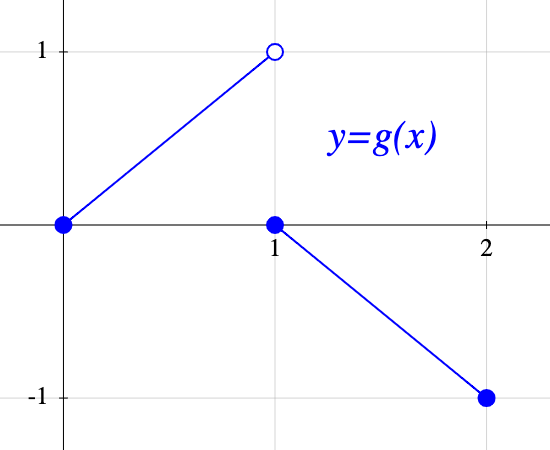
\includegraphics[scale=.35]{G20}
		\end{center}
	\end{frame}
	%-----------------------------

	%QUESTION_INFO: {"unit":7,"question":9,"title":"Trig suprema","images":[]}
	\begin{frame}[t]
		\frametitle{Trig suprema}

		Let $f(x) = \sin x$. \\ Find four open intervals $I_{1}$, $I_{2}$, $I_{3}$,
		$I_{4}$ such that

		\begin{enumerate}
			\item $f$ has a supremum and an infimum on $I_{1}$.

			\item $f$ has a supremum and no infimum on $I_{2}$.

			\item $f$ has a maximum and a minimum on $I_{3}$.

			\item $f$ has a maximum and no minimum on $I_{4}$.
		\end{enumerate}
	\end{frame}
	%-----------------------------

	%QUESTION_INFO: {"unit":7,"question":10,"title":"Empty set","images":[]}
	\begin{frame}[t]
		\frametitle{Empty set}

		\begin{enumerate}
			\item Does $\emptyset$ have an upper bound ?

			\item Does $\emptyset$ have a supremum?

			\item Does $\emptyset$ have a maximum?

			\item Is $\emptyset$ bounded above?
		\end{enumerate}
	\end{frame}

	%-----------------------------

	%QUESTION_INFO: {"unit":7,"question":11,"title":"Equivalent definitions of supremum","images":[]}
	\begin{frame}[t]
		\fontsize{13}{13}\selectfont
		\frametitle{Equivalent definitions of supremum}

		{\bfseries Assume $S$ is an upper bound of the set $A$.} \\ Which of the following
		is equivalent to ``$S$ is the supremum of $A$"?
		\vspace{.2cm}
		\begin{enumerate}
			\item If $R$ is an upper bound of $A$, \, then $S \leq R$.
				\vspace{.2cm}

			\item $\displaystyle \forall R \geq S$, \, $R$ is an upper bound of $A$.

			\item $\displaystyle \forall R \leq S$, \, $R$ is not an upper bound of
				$A$.

			\item $\displaystyle \forall R < S$, \, $R$ is not an upper bound of $A$.
				\vspace{.2cm}

			\item $\displaystyle \forall R < S$, \, $\displaystyle \exists x \in A$ \;
				such that \; $\displaystyle R < x$.

			\item $\displaystyle \forall R < S$, \, $\displaystyle \exists x \in A$ \;
				such that \; $\displaystyle R \leq x$.

			\item $\displaystyle \forall R < S$, \, $\displaystyle \exists x \in A$ \;
				such that \; $\displaystyle R < x \leq S$.

			\item $\displaystyle \forall R < S$, \, $\displaystyle \exists x \in A$ \;
				such that \; $\displaystyle R < x < S$.
				\vspace{.2cm}

			\item $\displaystyle \forall \varepsilon>0$, \; \,
				$\displaystyle \exists x \in A$ \; such that \;
				$\displaystyle S - \varepsilon < x$.

			\item $\displaystyle \forall \varepsilon>0$, \; \,
				$\displaystyle \exists x \in A$ \; such that \;
				$\displaystyle S - \varepsilon < x \leq S$.
		\end{enumerate}
	\end{frame}
	%-----------------------------

	%QUESTION_INFO: {"unit":7,"question":12,"title":"Fix these FALSE statements","images":[]}
	\begin{frame}[t]
		\fontsize{13}{13}\selectfont
		\frametitle{Fix these FALSE statements}

		\begin{enumerate}
			\item Let $f$ and $g$ be bounded functions on $[a,b]$. Then
				\[
					\; \substack{\text{ $\sup$ of $(f+g)$} \\ \text{on $[a,b]$} }\; \quad =
					\quad \; \substack{\text{ $\sup$ of $f$} \\ \text{on $[a,b]$} }\; \quad
					+ \quad \; \substack{\text{ $\sup$ of $g$} \\ \text{on $[a,b]$} }\;
				\]

				\vfill

			\item Let $a < b < c$. Let $f$ be a bounded function on $[a,c]$. Then
				\[
					\; \substack{\text{ $\sup$ of $f$} \\ \text{on $[a,c]$} }\; \quad = \quad
					\; \substack{\text{ $\sup$ of $f$} \\ \text{on $[a,b]$} }\; \quad + \quad
					\; \substack{\text{ $\sup$ of $f$} \\ \text{on $[b,c]$} }\;
				\]

				\vfill

			\item Let $f$ be a bounded function on $[a,b]$. Let $c \in \mathbb{R}$. Then:
				\[
					\; \substack{\text{ $\sup$ of $(cf)$} \\ \text{on $[a,b]$} }\; \quad =
					\quad c \; \left( \; \substack{\text{ $\sup$ of $f$} \\ \text{on $[a,b]$} }
					\; \right)
				\]
		\end{enumerate}
	\end{frame}
	%-----------------------------

	%QUESTION_INFO: {"unit":7,"question":13,"title":"True or False - Suprema and infima","images":[]}
	\begin{frame}[t]
		\fontsize{12}{12}\selectfont
		\frametitle{True or False - Suprema and infima}

		Let $A, B, C \subseteq \mathbb{R}$. Assume $C \subseteq A$. Which statements
		are true?
		\vspace{.1cm}

		If possible, fix the false statements
		\vspace{.2cm}
		\begin{enumerate}
			\item IF \;$A$ is bounded above, \; THEN \;$C$ is bounded above.

			\item IF \;$C$ is bounded below, \; THEN \;$A$ is bounded below.
				\vspace{.2cm}

			\item IF \;$A$ and $C$ are bounded above, \; THEN \;$\sup C \leq \sup A$.

			\item IF \;$A$ and $C$ are bounded below, \; THEN \;$\inf C \leq \inf A$.
				\vspace{.2cm}

			\item IF \;$A$ and $B$ are bounded, \;$\sup B \leq \sup A$, \;and \;$\inf A
				\leq \inf B$,
				\vspace{.1cm}

				THEN \;$B \subseteq A$.
				\vspace{.2cm}

			\item IF \;$A$ and $B$ are bounded above,
				\vspace{.1cm}

				THEN \;$\displaystyle \sup (A \cup B) =\max \{ \sup A, \sup B \}$.
				\vspace{.2cm}

			\item IF \;$A$ and $B$ are bounded above,
				\vspace{.1cm}

				THEN \;$\displaystyle \sup (A \cap B) =\min \{ \sup A, \sup B \}$.
		\end{enumerate}
	\end{frame}

	%-----------------------------

	%----------------------------------------------------------------------------------------

	%	The definition of definite integral

	%----------------------------------------------------------------------------------------

	%-----------------------------

	%QUESTION_INFO: {"unit":7,"question":14,"title":"Warm up: partitions","images":[]}
	\begin{frame}[t]
		\frametitle{Warm up: partitions}

		Which ones are partitions of $[0,2]$?

		\begin{enumerate}
			\item $\displaystyle [0,2]$

			\item $\displaystyle \{0.5, \,1, \,1.5\}$

			\item $\displaystyle \{0,\,2\}$

			\item $\displaystyle \{1,\,2\}$

			\item $\displaystyle \{0, \,e, \,2 \}$

			\item $\displaystyle \{0, \,1.5, \,1.6, \,1.7, \,1.8, \,1.9, \,2\}$

			\item $\displaystyle \left\{ \frac{n}{n+1}\; : \; n \in \mathbb{N}\right\}
				\cup \{ 2 \}$
		\end{enumerate}
	\end{frame}
	%-----------------------------

	%QUESTION_INFO: {"unit":7,"question":15,"title":"Partitions of different intervals","images":[]}
	\begin{frame}[t]
		\fontsize{13}{13}\selectfont
		\frametitle{Partitions of different intervals}

		Let $a<b<c$. Which of these statements are true?

		If any are false, fix them.
		\vspace{.1cm}
		\begin{enumerate}
			\item IF $P$ and $Q$ are partitions of $[a,b]$,
				\vspace{.1cm}

				THEN $P \cup Q$ is a partition of $[a,b]$.
				\vspace{.1cm}

			\item IF $P$ and $Q$ are partitions of $[a,b]$,
				\vspace{.1cm}

				THEN $P \cap Q$ is a partition of $[a,b]$.
				\vspace{.1cm}

			\item IF $P$ is a partition of $[a,b]$ and $Q$ is a partition of $[b,c]$
				\vspace{.1cm}

				THEN $P \cup Q$ is a partition of $[a,c]$
				\vspace{.1cm}

			\item IF $P$ is a partition of $[a,c]$,
				\vspace{.1cm}

				THEN $P \cap [a,b]$ is a partition of $[a,b]$
		\end{enumerate}
	\end{frame}
	%-----------------------------

	%QUESTION_INFO: {"unit":7,"question":16,"title":"Warm up: lower and upper sums","images":[]}
	\begin{frame}[t]
		\frametitle{Warm up: lower and upper sums}

		Let $\displaystyle f(x) = \sin x$.

		Consider the partition $\displaystyle P= \{0, 1, 3\}$ of the interval
		$\displaystyle [0,3]$.

		Calculate $\displaystyle L_{P}(f)$ and $\displaystyle U_{P}(f)$.
	\end{frame}

	%-----------------------------

	%QUESTION_INFO: {"unit":7,"question":17,"title":"Equations for lower and upper sums","images":[]}
	\begin{frame}[t]
		\fontsize{13}{13}\selectfont
		\frametitle{Equations for lower and upper sums}

		Let $f$ be a {\bfseries decreasing}, bounded function on $[a,b]$. \\ Let $\displaystyle
		P = \{x_{0}, x_{1}, \ldots, x_{N}\}$ be a partition of $[a,b]$

		Which ones are a valid equation for $L_{P}(f)$? For $U_{P}(f)$?

		\begin{multicols}{3}
			\begin{enumerate}
				\item $\displaystyle \sum_{i=0}^{N}f(x_{i}) \, \Delta x_{i}$

				\item $\displaystyle \sum_{i = 1}^{N}f(x_{i}) \, \Delta x_{i}$

				\item $\displaystyle \sum_{i = 0}^{N-1}f(x_{i}) \, \Delta x_{i}$

				\item $\displaystyle \sum_{i = 1}^{N}f(x_{i+1}) \, \Delta x_{i}$

				\item $\displaystyle \sum_{i = 1}^{N}f(x_{i-1}) \, \Delta x_{i}$

				\item $\displaystyle \sum_{i = 0}^{N-1}f(x_{i}) \, \Delta x_{i+1}$
			\end{enumerate}
		\end{multicols}

		Recall: $\displaystyle \Delta x_{i}= x_{i}- x_{i-1}$.
	\end{frame}
	%------------------------------

	%QUESTION_INFO: {"unit":7,"question":18,"title":"Easier than it looks","images":[]}
	\begin{frame}[t]
		\frametitle{Easier than it looks}

		Let $f$ be a bounded function on $[a,b]$. \\ Assume $f$ is not constant. \\
		Prove that there exists a partition $P$ of $[a,b]$ such that
		\[
			L_{P}(f) \neq U_{P}(f).
		\]
	\end{frame}
	%-----------------------------

	%QUESTION_INFO: {"unit":7,"question":19,"title":"Joining partitions","images":[]}
	\begin{frame}[t]
		\frametitle{Joining partitions}

		Assume
		\begin{align*}
			L_{P}(f)=2, & \quad U_{P}(f)=6 \\
			L_{Q}(f)=3, & \quad U_{Q}(f)=8
		\end{align*}

		\begin{enumerate}
			\item Is $\displaystyle P \subseteq Q$?

			\item Is $\displaystyle Q \subseteq P$?

			\item What can you say about $\displaystyle L_{P \cup Q}(f) \text{ and }U_{P
				\cup Q}(f)$?
		\end{enumerate}
	\end{frame}
	%-----------------------------

	%QUESTION_INFO: {"unit":7,"question":20,"title":"A tricky question","images":[]}
	\begin{frame}[t]
		\fontsize{13}{13}\selectfont
		\frametitle{A tricky question}

		Let $f$ be a bounded function on $[a,b]$. Which statement is true?

		\begin{enumerate}
			\item There exists a partition $P$ of $[a,b]$ such that
				\[
					\underline{I_a^b}(f)=L_{P}(f) \quad \quad \text{and}\quad \quad \overline
					{I_a^b}(f)=U_{P}(f).
				\]

			\item There exist partitions $P$ and $Q$ of $[a,b]$ such that
				\[
					\underline{I_a^b}(f)=L_{P}(f) \quad \quad \text{and}\quad \quad \overline
					{I_a^b}(f)=U_{Q}(f).
				\]
			% \pause

			\item There exists a partition $P$ of $[a,b]$ such that
				\[
					\underline{I_a^b}(f)=L_{P}(f).
				\]
		\end{enumerate}

		\begin{center}
			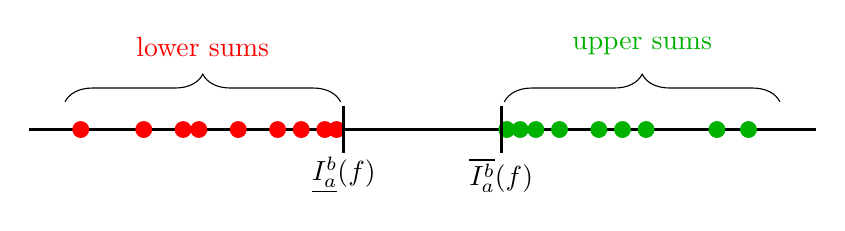
\begin{tikzpicture}
				\draw[thick] (-5,0) to (5,0);

				\draw[decorate, decoration={brace, amplitude=10pt}, yshift=10pt]
					(-1.04-3.5,-0) -- (-1.04-0,-0)
					node[red, midway, yshift=20pt] {lower sums};

				\draw[red, fill] (-1.04-2.5,0) circle[radius=0.1];
				\draw[red, fill] (-1.04-3.3,0) circle[radius=0.1];
				\draw[red, fill] (-1.04-2.0,0) circle[radius=0.1];
				\draw[red, fill] (-1.04-1.8,0) circle[radius=0.1];
				\draw[red, fill] (-1.04-1.3,0) circle[radius=0.1];
				\draw[red, fill] (-1.04-0.8,0) circle[radius=0.1];
				\draw[red, fill] (-1.04-0.5,0) circle[radius=0.1];
				\draw[red, fill] (-1.04-0.2,0) circle[radius=0.1];
				\draw[red, fill] (-1.04-0.05,0) circle[radius=0.1];

				\draw[decorate, decoration={brace, amplitude=10pt}, yshift=10pt]
					(1.04+0,0) -- (1.04+3.5,0)
					node[verde, midway, yshift=20pt] {upper sums};

				\draw[verde, fill] (1.04+2.7,0) circle[radius=0.1];
				\draw[verde, fill] (1.04+3.1,0) circle[radius=0.1];
				\draw[verde, fill] (1.04+1.8,0) circle[radius=0.1];
				\draw[verde, fill] (1.04+1.5,0) circle[radius=0.1];
				\draw[verde, fill] (1.04+1.2,0) circle[radius=0.1];
				\draw[verde, fill] (1.04+0.7,0) circle[radius=0.1];
				\draw[verde, fill] (1.04+0.4,0) circle[radius=0.1];
				\draw[verde, fill] (1.04+0.2,0) circle[radius=0.1];
				\draw[verde, fill] (1.04+0.03,0) circle[radius=0.1];
				\draw[very thick, black]
					(-1,0.3) to (-1,-0.3)
					node[yshift=-8pt] {$\underline{I_a^b}(f)$};
				\draw[very thick, black]
					(1,0.3) to (1,-0.3)
					node[yshift=-8pt] {$\overline{I_a^b}(f)$};
			\end{tikzpicture}
		\end{center}
	\end{frame}
	%-----------------------------

	%QUESTION_INFO: {"unit":7,"question":21,"title":"An alternative definition","images":[]}
	\begin{frame}[t]
		\fontsize{13}{13}\selectfont
		\frametitle{An alternative definition}

		Let $f$ be a bounded function on the interval $[a,b]$. Let
		$M \in \mathbb{R}$.

		Some of these four statements imply others. What implies what?
		\vspace{.2cm}
		\begin{enumerate}
			\item $\forall$ partition $P$ of $[a,b]$, \;
				$\displaystyle L_{P}(f) \,\leq\, M$,
				\vspace{.2cm}

			\item $\forall \varepsilon>0$, $\exists$ partition $P$ of $[a,b]$ \; s.t. \;
				$\displaystyle M - \varepsilon \,< \, L_{P}(f)$
				\vspace{.2cm}

			\item $\displaystyle M \, \leq \, \underline{I_a^b}(f)$

			\item $\displaystyle \underline{I_a^b}(f) \, \leq \, M$
		\end{enumerate}

		% \pause
		\vfill

		Based on this exercise, we could have defined $\underline{I_a^b}(f)$ as \\``the
		only number $M \in \mathbb{R}$ satisfying these two properties: ..."

		Use the same idea to write an alternative definition of $\overline{I_a^b}(f)$.

		\vfill
	\end{frame}
	%------------------------------

	%QUESTION_INFO: {"unit":7,"question":22,"title":"The “$\\varepsilon$—characterization” of integrability","images":[]}
	\begin{frame}[t]
		\fontsize{11}{11}\selectfont
		\frametitle{The ``$\varepsilon$--characterization" of integrability}

		\begin{block}{\fontsize{11}{11}\selectfont True or False?}
			Let $f$ be a bounded function on $[a,b]$.
			\begin{enumerate}
				\item IF \hfill ``$\forall \varepsilon>0$, $\exists$ a partition $P$ of
					$[a,b]$ s.t. $\displaystyle U_{P}(f) - L_{P}(f) < \varepsilon$",
					\vspace{.1cm}

					THEN \; $f$ is integrable on $[a,b]$
					\vspace{.1cm}

				\item IF \quad \quad \, $f$ is integrable on $[a,b]$
					\vspace{.1cm}
					\\
					\vspace{.1cm}

					THEN \hfill ``$\forall \varepsilon>0$, $\exists$ a partition $P$ of $[a
					,b]$ s.t. $\displaystyle U_{P}(f) - L_{P}(f) < \varepsilon$".
					\vspace{.1cm}
			\end{enumerate}
		\end{block}

		\vfill

		\begin{center}
			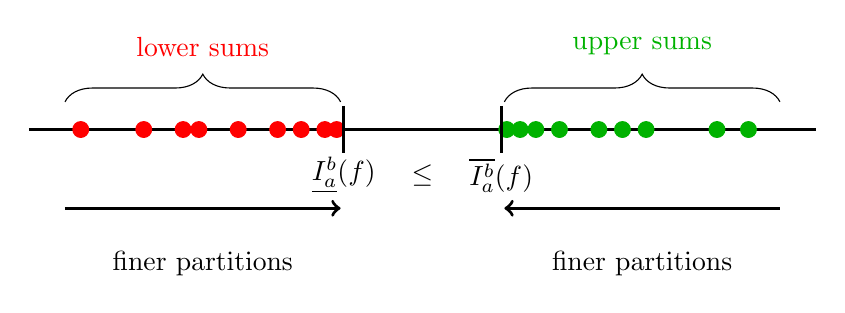
\begin{tikzpicture}
				\draw[thick] (-5,0) to (5,0);

				\draw[decorate, decoration={brace, amplitude=10pt}, yshift=10pt]
					(-1.04-3.5,-0) -- (-1.04-0,-0)
					node[red, midway, yshift=20pt] {lower sums};

				\draw[red, fill] (-1.04-2.5,0) circle[radius=0.1];
				\draw[red, fill] (-1.04-3.3,0) circle[radius=0.1];
				\draw[red, fill] (-1.04-2.0,0) circle[radius=0.1];
				\draw[red, fill] (-1.04-1.8,0) circle[radius=0.1];
				\draw[red, fill] (-1.04-1.3,0) circle[radius=0.1];
				\draw[red, fill] (-1.04-0.8,0) circle[radius=0.1];
				\draw[red, fill] (-1.04-0.5,0) circle[radius=0.1];
				\draw[red, fill] (-1.04-0.2,0) circle[radius=0.1];
				\draw[red, fill] (-1.04-0.05,0) circle[radius=0.1];

				\draw[decorate, decoration={brace, amplitude=10pt}, yshift=10pt]
					(1.04+0,0) -- (1.04+3.5,0)
					node[verde, midway, yshift=20pt] {upper sums};

				\draw[verde, fill] (1.04+2.7,0) circle[radius=0.1];
				\draw[verde, fill] (1.04+3.1,0) circle[radius=0.1];
				\draw[verde, fill] (1.04+1.8,0) circle[radius=0.1];
				\draw[verde, fill] (1.04+1.5,0) circle[radius=0.1];
				\draw[verde, fill] (1.04+1.2,0) circle[radius=0.1];
				\draw[verde, fill] (1.04+0.7,0) circle[radius=0.1];
				\draw[verde, fill] (1.04+0.4,0) circle[radius=0.1];
				\draw[verde, fill] (1.04+0.2,0) circle[radius=0.1];
				\draw[verde, fill] (1.04+0.03,0) circle[radius=0.1];
				\draw[very thick, ->]
					(-1.04-3.5,-1) -- (-1.04-0,-1)
					node[black, midway, yshift=-20pt] {finer partitions};
				\draw[very thick, ->]
					(1.04+3.5,-1) -- (1.04+0,-1)
					node[black, midway, yshift=-20pt] {finer partitions};
				\draw[very thick, black]
					(-1,0.3) to (-1,-0.3)
					node[yshift=-8pt] {$\underline{I_a^b}(f)$};
				\draw[very thick, black]
					(1,0.3) to (1,-0.3)
					node[yshift=-8pt] {$\overline{I_a^b}(f)$};
				\node[yshift=-8pt] at (0,-0.3) {$\leq$};
			\end{tikzpicture}
		\end{center}
	\end{frame}
	%------------------------------

	%QUESTION_INFO: {"unit":7,"question":23,"title":"The “$\\varepsilon$—characterization” of integrability - Part 1","images":[]}
	\begin{frame}[t]
		\fontsize{11}{11}\selectfont
		\frametitle{The ``$\varepsilon$--characterization" of integrability - Part 1}

		\begin{block}{\fontsize{11}{11}\selectfont True or False?}
			Let $f$ be a bounded function on $[a,b]$.
			\begin{itemize}
				\item IF \hfill ``$\forall \varepsilon>0$, $\exists$ a partition $P$ of
					$[a,b]$ s.t. $\displaystyle U_{P}(f) - L_{P}(f) < \varepsilon$",

				\item THEN \; $f$ is integrable on $[a,b]$
			\end{itemize}
		\end{block}

		\emph{Hints:}
		\begin{enumerate}
			\item Recall the definition of ``$f$ is integrable on $[a,b]$".

			\item Let $P$ be a partition. \\ Order the numbers
				$\displaystyle U_{P}(f)$, $\displaystyle L_{P}(f)$,
				$\displaystyle \overline{I_a^b}(f)$, $\displaystyle \underline{I_a^b}(f)$.
				\\ (Draw a picture of these numbers in the real line.)
		\end{enumerate}
	\end{frame}
	%------------------------------

	%QUESTION_INFO: {"unit":7,"question":24,"title":"The “$\\varepsilon$—characterization” of integrability - Part 2","images":[]}
	\begin{frame}[t]
		\fontsize{11}{11}\selectfont
		\frametitle{The ``$\varepsilon$--characterization" of integrability - Part 2}

		\begin{block}{\fontsize{11}{11}\selectfont True or False?}
			Let $f$ be a bounded function on $[a,b]$.
			\begin{itemize}
				\item IF \quad \quad \, $f$ is integrable on $[a,b]$

				\item THEN \hfill ``$\forall \varepsilon>0$, $\exists$ a partition $P$
					of $[a,b]$ s.t. $\displaystyle U_{P}(f) - L_{P}(f) < \varepsilon$".
			\end{itemize}
		\end{block}

		\emph{Hints:} Assume $f$ is integrable on $[a,b]$. Let $I$ be the integral. Fix
		$\varepsilon>0$.
		\begin{enumerate}
			\item Recall the definition of ``$f$ is integrable on $[a,b]$".

			\item There exist a partition $P_{1}$ s.t.
				$\displaystyle U_{P_1}(f) < I + \frac{\varepsilon}{2}$. Why?

			\item There exist a partition $P_{2}$ s.t.
				$\displaystyle L_{P_2}(f) > I - \frac{\varepsilon}{2}$. Why?

			\item What can you say about $\displaystyle U_{P_1}(f) - L_{P_2}(f)$?
				\vspace{.1cm}

			\item Construct a partition $P$ s.t.
				$\displaystyle L_{P_2}(f) \leq L_{P}(f) \leq U_{P}(f) \leq U_{P_1}(f)$.
		\end{enumerate}
	\end{frame}
	%------------------------------

	%QUESTION_INFO: {"unit":7,"question":25,"title":"Example 1: a constant function","images":[]}
	\begin{frame}[t]
		\fontsize{13}{13}\selectfont
		\frametitle{Example 1: a constant function}

		Consider the function \; $f(x)=2$ \; on \; $[0,4]$.
		\vspace{.2cm}

		\begin{enumerate}
			\item Given $\displaystyle P =\{ 0, 1, e, \pi, 4 \}$, compute
				$\displaystyle L_{P}(f)$ and $\displaystyle U_{P}(f)$.

			\item Explicitly compute \emph{all} the upper sums and \emph{all} the lower
				sums.
				\vspace{.2cm}

			\item Compute $\displaystyle \overline{I_0^4}(f)$
				\vspace{.2cm}

			\item Compute $\displaystyle \underline{I_0^4}(f)$
				\vspace{.2cm}

			\item Is $f$ integrable on $[0,4]$?
		\end{enumerate}
	\end{frame}
	%------------------------------

	%QUESTION_INFO: {"unit":7,"question":26,"title":"Example 2: a non-continuous function","images":[]}
	\begin{frame}[t]
		\fontsize{13}{13}\selectfont
		\frametitle{Example 2: a non-continuous function}

		Consider the function \; $\displaystyle f(x) =
		\begin{cases}
			0 & x = 0        \\
			5 & 0 < x \leq 1
		\end{cases}$, \;defined on $[0,1]$.

		\begin{enumerate}
			\item Let $\displaystyle P = \{0, 0.2, 0.5, 0.9, 1 \}$.
				\vspace{.1cm}

				Calculate $\displaystyle L_{P}(f)$ and $\displaystyle U_{P}(f)$ for this
				partition.
				\vspace{.1cm}

			\item Fix an arbitrary partition $P = \{x_{0}, x_{1}, \dots, x_{N}\}$ of $[
				0,1]$. \\
				\vspace{.1cm}

				What is $U_{P}(f)$? What is $\displaystyle L_{P}(f)$? (Draw a picture!)
				\vspace{.1cm}

			\item Find a partition $P$ with exactly 3 points (2 subintervals) such that
				$\displaystyle L_{P}(f) = 4.99$.

			\item What is the upper integral, $\overline{I_0^1}(f)$?

			\item What is the lower integral, $\underline{I_0^1}(f)$?

			\item Is $f$ integrable on $[0,1]$?
		\end{enumerate}
	\end{frame}

	%------------------------------

	%QUESTION_INFO: {"unit":7,"question":27,"title":"Example 3: a very non-continuous function","images":[]}
	\begin{frame}[t]
		\fontsize{13}{13}\selectfont
		\frametitle{Example 3: a very non-continuous function}

		Consider the function $f$ defined on $[0,1]$:
		\[
			f(x) =
			\begin{cases}
				1/2 & \text{ if } 0 \leq x \leq 1/2                               \\
				1   & \text{ if } 1/2 < x \leq 1 \text{ and } x \in \mathbb{Q}    \\
				0   & \text{ if } 1/2 < x \leq 1 \text{ and } x \notin \mathbb{Q}
			\end{cases}
		\]

		\begin{enumerate}
			\item Draw a picture!

			\item Let $\displaystyle P= \{ 0, 0.2, 0.4, 0.6, 0.8, 1 \}$. Calculate
				$\displaystyle L_{P}(f)$ and $\displaystyle U_{P}(f)$.

			\item Construct a partition $P$ such that $\displaystyle L_{P}(f) = \frac{1}{4}$
				and $\displaystyle U_{P}(f) = \frac{3}{4}$

			\item What is the upper integral, $\overline{I_0^1}(f)$?

			\item What is the lower integral, $\underline{I_0^1}(f)$?

			\item Is $f$ integrable on $[0,1]$?
		\end{enumerate}
	\end{frame}
	%-----------------------------

	%QUESTION_INFO: {"unit":7,"question":28,"title":"Sum of non-integrable functions","images":[]}
	\begin{frame}[t]
		\frametitle{Sum of non-integrable functions}

		Find bounded functions $f$ and $g$ on $[0,1]$ such that
		\begin{itemize}
			\item $f$ is non-integrable on $[0,1]$,

			\item $g$ is non-integrable on $[0,1]$,

			\item $f+g$ is integrable on $[0,1]$.
		\end{itemize}
		or prove this is impossible.
	\end{frame}
	%-----------------------------

	%QUESTION_INFO: {"unit":7,"question":29,"title":"Properties of the integral","images":[]}
	\begin{frame}
		\fontsize{13}{13}\selectfont
		\frametitle{Properties of the integral}

		Assume we know the following
		\begin{align*}
			 & \int_{0}^{2}f(x) dx = 3, &  & \int_{0}^{4}f(x) dx = 9, &  & \int_{0}^{4}g(x) dx = 2.
		\end{align*}

		Compute:
		\begin{multicols}{2}
			\begin{enumerate}
				\item $\displaystyle \int_{0}^{2}f(t) dt$

				\item $\displaystyle \int_{0}^{2}f(x) dx$

				\item $\displaystyle \int_{0}^{2}f(t) dx$

				\item $\displaystyle \int_{2}^{0}f(x) dx$

				\item $\displaystyle \int_{2}^{4}f(x) dx$

				\item $\displaystyle \int_{-2}^{0}f(x) dx$

				\item $\displaystyle \int_{0}^{4}\left[ f(x) - 2g(x) \right] \; dx$
			\end{enumerate}
		\end{multicols}
		\vfill
	\end{frame}
	%------------------------------

	%QUESTION_INFO: {"unit":7,"question":30,"title":"The norm of a partition","images":[]}
	\begin{frame}[t]
		\fontsize{13}{13}\selectfont
		\frametitle{The norm of a partition}

		\begin{enumerate}
			\item Construct a partition $P$ of $[0,1]$ such that $\displaystyle ||P|| =
				\frac{\pi}{10}$.

			\item Construct a sequence of partitions of $[0,1]$
				\[
					P_{1}, P_{2}, P_{3}, \ldots
				\]
				\emph{as simple as possible}, such that $\displaystyle \lim_{n \to
				\infty}||P_{n}|| = 0$.

			\item Construct a \emph{different} sequence of partitions of $[0,1$]
				\[
					Q_{1}, Q_{2}, Q_{3}, \ldots
				\]
				such that $\displaystyle \lim_{n \to \infty}||Q_{n}|| = 0$.
		\end{enumerate}
	\end{frame}
	%------------------------------

	%QUESTION_INFO: {"unit":7,"question":31,"title":"Compute $\\displaystyle \\int_{1}^{2} \\! x^{2} dx$ using Riemann sums","images":[]}
	\begin{frame}[t]
		\fontsize{13}{13}\selectfont
		\frametitle{Compute $\displaystyle \int_{1}^{2}\! x^{2}dx$ using Riemann
		sums}

		\begin{block}{}
			Let $\displaystyle f(x) = x^{2}$ on $[1,2]$. Let $P_{n}$ be the partition
			that breaks $[1,2]$ into $n$ subintervals of equal length.
			\begin{enumerate}
				\item Write a explicit formula for $P_{n}$.

				\item What is $\Delta x_{i}$?

				\item Write the Riemann sum $\displaystyle S^{*}_{P_n}(f)$ with sigma notation
					\\ (choose $x^{*}_{i}$ as the right endpoint).

				\item Add the sum

				\item Compute $\displaystyle \lim_{n \to \infty}S^{*}_{P_n}(f)$.

				\item Repeat the last 3 questions when we choose $x^{*}_{i}$ as the left
					endpoint.
			\end{enumerate}
		\end{block}
		{\fontsize{10}{10}\selectfont \emph{Helpful identities:} $\displaystyle \quad \sum_{i=1}^{N}i = \frac{N(N+1)}{2}, \quad \quad \sum_{i=1}^{N}i^{2}= \frac{N(N+1)(2N+1)}{6}$ }
	\end{frame}
	%------------------------------

	%QUESTION_INFO: {"unit":7,"question":32,"title":"Riemann sums backwards","images":[]}
	\begin{frame}[t]
		\frametitle{Riemann sums backwards}

		Interpret the following limits as integrals:
		\begin{enumerate}
			\begin{multicols}{2}
				\item $\displaystyle \lim_{n \to \infty}\sum_{i=1}^{n}\frac{1}{n}\sin \frac{i}{n}$
				\item $\displaystyle \lim_{n \to \infty}\sum_{i=1}^{n}\frac{n+i}{n^{2}}$
			\end{multicols}
		\end{enumerate}
		{\fontsize{10}{10}\selectfont \emph{Hint:} Let $f$ be a continuous function on $[0,1]$. Write a formula for $\displaystyle \int_{0}^{1}f(x) dx$ as a limit of Riemann sums, making the simplest choices you can. }
	\end{frame}
	%------------------------------

	%QUESTION_INFO: {"unit":7,"question":33,"title":"The Mean Value Theorem for integrals","images":[]}
	\begin{frame}[t]
		\fontsize{13}{13}\selectfont
		\frametitle{The Mean Value Theorem for integrals}

		Prove the following theorem.

		\begin{block}{\fontsize{13}{13}\selectfont Theorem}
			Let $a < b$. Let $f$ be a continuous function on $[a,b]$. \\ There exists $c
			\in [a,b]$ such that
			\vspace{-.5cm}
			\[
				f(c) \; = \; \frac{1}{b-a}\int_{a}^{b}f(t) dt
			\]
		\end{block}

		% \pause

		\emph{Hints:}
		\begin{enumerate}
			\item Compute $L_{P}(f)$ and $U_{P}(f)$ for the partition $\displaystyle P=
				\{a,b\}$.

			\item Use that $\displaystyle L_{P}(f) \leq \int_{a}^{b}f(t)dt \leq U_{P}(f
				)$ to prove that
				\vspace{-.6cm}
				\
				\[
					??? \; \leq \; \frac{1}{b-a}\int_{a}^{b}f(t) dt \; \leq \; \; ???
				\]
				\vspace{-.6cm}

			\item Use EVT and IVT.
		\end{enumerate}
	\end{frame}
	%-----------------------------

	%-----------------------------
\end{document}
%-----------------------------

%-----------------------------